\chapter{Search for Charged Higgs Bosons}\label{chap:hpana}
	This chapter details a search for a charged Higgs boson decaying to a hadronically decaying tau lepton and a neutrino; the phenomenology is discussed in Section \ref{sec:Hpm}. This search contains two subchannels, \taujets and \taulep based on the decay of the  associated top quark in the collision event. The \taujets subchannel ($t\rightarrow Wb, \, W \rightarrow q\bar{q}$)  has a higher branching fraction, leading to higher sensitivity at larger \mHpm values. The \taulep subchannel ($t\rightarrow Wb, \, W \rightarrow \ell \nu$)  has a much lower branching fraction, but takes advantage of single-lepton triggers which enhance background suppression of QCD $\mathrm{jet} \, \rightarrow \, \tau$ fakes. This leads to an increased sensitivity at lower \mHpm values. The extra neutrino in the \taulep decay mode creates extra difficulties in separating signal from background in this subchannel by adding a significant contribution to the \Etm calculation for the event. 

	This chapter discusses in detail the entire analysis, including the signal signatures, event selections, analyzed datasets, modelling of backgrounds, analysis strategy, studies of systematic uncertainties, and results.

	\section{Signature and Event Selection}\label{sec:signal}
		As shown in Figure \ref{fig:hpm-diagrams}, the production of the \Hpm is dependent on the mass \mHpm. Table \ref{tab:hplus-production} shows the production mechanisms for \mHpm values with respect to the top quark mass $m_t$ as well as the main decay mode (and theoretical constraints), as well as the main source of background. Three mass ranges are defined, low mass $80 \leq \mHpm \leq 130 $ GeV, intermediate mass $140 \leq \mHpm \leq 190$, and high mass $200 \leq \mHpm \leq 3000$ GeV.  The two subchannels have similar signal signatures with a hard scatter source of \Etm, one \tauhad, and at least 1 \bjet from the associated top decay. In the \taulep subchannel there is an extra requirement of a lepton (e or $\mu$). Due to the variable amount of energy available to the final state products based on \mHpm the event topology changes as a function of \mHpm. As described in Section \ref{ssec:mva}, classifiers are trained and evaluated in \mHpm bins to account for the varying event topology.

		\begin{table}[!thp]
			\centering
			\resizebox{\textwidth}{!}{
			\begin{tabular}{| c | c | c | c |}
			\hline
			\textbf{\Hpm Mass} & \textbf{Production Mechanism} & \textbf{Decay}  & \textbf{Main Background}\\
			\hline \hline
			\multicolumn{1}{|c|}{\multirow{2}{*}{$\mHpm < m_{t}$}} 		& \begin{tabular}[c]{@{}c@{}} double-resonant $t \rightarrow H^\pm b$ (LO) \\ 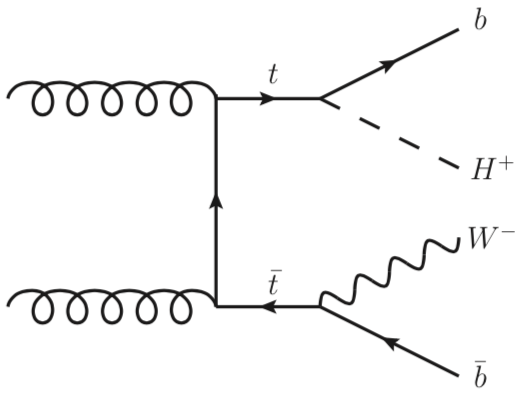
\includegraphics[width=.19\textwidth]{chapters/chapter6_HPlus/images/double_resonant_production_low_mass.png} \end{tabular} 											& \begin{tabular}[c]{@{}c@{}} \HpmLong \\ (low $\tanb \implies$ $\Hpm \rightarrow cs$ or $\Hpm \rightarrow cb$ ) \end{tabular} 																	& \ttbar, single-top \\ \hline

			\multicolumn{1}{|c|}{\multirow{3}{*}{$\mHpm \simeq m_{t}$}} & \begin{tabular}[c]{@{}c@{}} non-resonant $t \rightarrow \Hpm b$ (LO) \\ 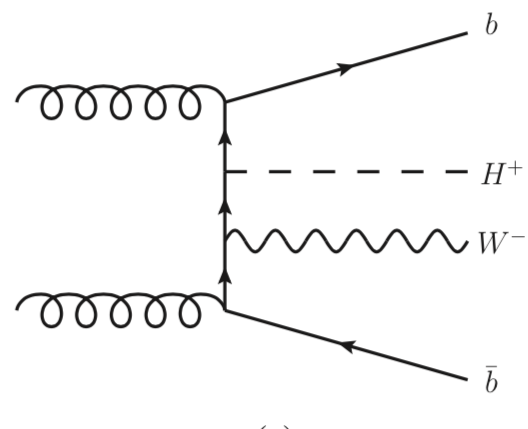
\includegraphics[width=.19\textwidth]{chapters/chapter6_HPlus/images/non_resonant_production_intermediate_mass.png} \\ interferences taken into account \end{tabular} 	& $\Hpm \rightarrow \tau \nu$  																																									& \ttbar, single-top \\ \hline

			\multicolumn{1}{|c|}{\multirow{3}{*}{$\mHpm > m_{t}$}}		& \begin{tabular}[c]{@{}c@{}} single-resonant $gg \rightarrow tbH^\pm$ (NLO) \\ 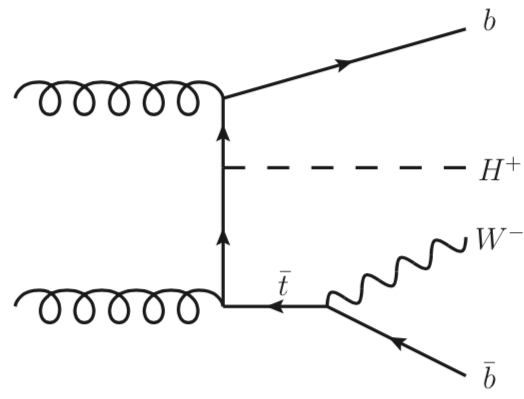
\includegraphics[width=.19\textwidth]{chapters/chapter6_HPlus/images/single_resonant_production_large_mass.png} \end{tabular} 										& \begin{tabular}[c]{@{}c@{}} $\Hpm \rightarrow tb$ \\ ($cos(\beta-\alpha) \simeq 0$ and large $tan(\beta) \implies \Hpm \rightarrow \tau \nu$ \\ $BR(\HpmLong) \simeq 10-15\%$ ) \end{tabular} & multi-jet \\ \hline

			\end{tabular}}
			\caption{\Hpm production mechanisms based on \mHpm, dominant \Hpm decay mode, and the main background associated with the diagram.}
			\label{tab:hplus-production}
		\end{table}

		\subsection{Object Definitions}\label{ssec:object-def}
		Table \ref{tab:object-defs} shows the identification requirements on all objects used in the analysis. In both subchannels \tauhad candidates are required to fit the medium working point described in Section \ref{ssec:reco-tau} that corresponds to a 75\% efficiency for 1-prong and 60\% efficiency for 3-prong \tauhad identification, an $\abs{\eta}$ cut of $< 2.3$ that also excludes the gap and crack region of the ATLAS calorimeters at $1.37 < \abs{\eta} < 1.52$, an overlap removal with electrons is also performed. For the \taujets subchannel, the \tauhad \pt is required to be greater than 40 GeV and greater than 30 GeV for the \taulep subchannel. Although muons and electrons are not part of the \taujets signal final state, a loose identification and isolation requirement is used to veto events; while the \taulep subchannel requires there to be either an electron or a muon that passes the tight identification and isolation requirements as well as a \pt above 30 GeV. The jets in candidate events are required to have greater than 25 GeV in \pt and are made with the anti-$k_t$ algorithm with R=0.4. Jets tagged as \bjets are done so at a 70\% efficient working point using the DL1r tagger described in Section \ref{ssec:flavor-tagging}.

		\begin{table}[!thp]
			\centering
			\resizebox{\textwidth}{!}{
			\begin{tabular}{| c | l | l |}
			\hline
			Object & \textbf{\taujets} & \textbf{\taulep} \\
			\hline \hline
			\multicolumn{1}{|c|}{\multirow{3}{*}{\tauhad}} & \begin{tabular}[c]{@{}c@{}}Leading reconstructed $\tau$ (regardless of its ID), \\ mediumID$^{*}$, $\pt > 40$ GeV, $\abs{\eta}^{***} < 2.3$, $e$ OLR \end{tabular} & \begin{tabular}[c]{@{}c@{}} Leading reconstructed $\tau$ (regardless of its ID), \\ mediumID$^{*}$, $\pt > 30$ GeV, $\abs{\eta}^{***} < 2.3$, $e$ OLR \end{tabular} \\[4ex] \hline
			\multicolumn{1}{|c|}{\multirow{3}{*}{$e$}} & \begin{tabular}[c]{@{}c@{}} LoseLLH, $\pt > 20$ GeV, $\abs{\eta}^{***} < 2.47$, \\ Loose isolation, IP cuts \end{tabular} &  \begin{tabular}[c]{@{}c@{}} TightLLH, $\pt > 30$ GeV, $\abs{\eta}^{***} < 2.47$, \\ Tight isolation, IP cuts \end{tabular} \\[4ex] \hline
			\multicolumn{1}{|c|}{\multirow{3}{*}{$\mu$}} & \begin{tabular}[c]{@{}c@{}} LooseID, $\pt > 20$ GeV, $\abs{\eta} < 2.5$, \\Loose isolation, IP cuts \end{tabular} & \begin{tabular}[c]{@{}c@{}} TightID, $\pt > 30$ GeV, $\abs{\eta} < 2.5$,\\ Tight isolation, IP cuts \end{tabular} \\[4ex] \hline 
			\multicolumn{1}{|c|}{\multirow{3}{*}{jet}} & \begin{tabular}[c]{@{}c@{}} AntiKt4EMPFlow, $\pt > 25$, GeV $\abs{\eta} < 2.5$,\\ JVT$^{**}$  $> 0.59$, Btag=70\%, DL1r \end{tabular} & \begin{tabular}[c]{@{}c@{}} AntiKt4EMPFlow, $\pt > 25$ GeV, $\abs{\eta} <2.5$, \\ JVT$^{**}$  $ > 0.59$ , Btag=70\%, DL1r \end{tabular} \\[4ex] \hline
			\end{tabular}}
			\caption{Definitions of physics objects used in this analysis.}
			\label{tab:object-defs}
		\end{table}

		% \begin{columns}
		% \column{.3\textwidth}
		% \begin{itemize}
		%   \footnotesize
		%   \item $\tau$ mediumID$^{*}$
		%   \begin{itemize}
		%     \tiny
		%     \item 1-prong: 75\% ID eff 
		%     \item 3-prong: 60\% ID eff
		%   \end{itemize}
		% \end{itemize}
		% \column{.3\textwidth}
		% \begin{itemize}
		%   \footnotesize
		%   \item JVT$^{**}$
		%     \begin{itemize}
		%       \tiny
		%       \item $\pt < 60$ GeV
		%       \item $\abs{\eta}<2.4$
		%   \end{itemize}
		% \end{itemize}
		% \column{.3\textwidth}
		% \begin{itemize}
		%   \footnotesize
		%   \item $\abs{\eta}^{***}$
		%     \begin{itemize}
		%       \tiny
		%       \item $1.37 < \abs{eta} < 1.52 $ excluded
		%   \end{itemize}
		% \end{itemize}
		% \end{columns}

		\subsection{Event Selections}\label{ssec:event-selection}
			Each subchannel signal region has stricter requirements than those described in Section \ref{tab:object-defs}. Table \ref{tab:signal-regions} details these selections. The channels differ in the triggers used; the \taujets subchannel relies on \Etm triggers while the \taulep subchannel relies on single lepton triggers. Due to the difficulty of separating signal from background the \taujets subchannel has a higher \pt cut on the \tauhad of 40 GeV as opposed to the \taulep value of 30 GeV. In addition, a higher value of \Etm of 150 GeV is required for the \taujets subchannel. A value of 50 GeV is also required of the transverse mass $m_{T}$ defined as 
			\begin{equation}\label{eqn:transverse-mass}
			m_{T} = \sqrt{ 2 \pt^{\tau} \Etm (1 - cos \Delta \phi_{\tau,\Etm}) }
			\end{equation}
			The \taulep has no such requirement, but does require the \tauhad and lepton to have opposite electromagnetic charge. A set of orthogonal control regions are defined for each subchannel to verify proper background modelling and are described in Section \ref{sec:bkg-modeling}. The acceptance of signal in the signal regions defined in \ref{tab:signal-regions} is shown in Figure \ref{fig:signal-acceptance}.


			\begin{table}[!thp]
				\centering
				\resizebox{.75\textwidth}{!}{
				\begin{tabular}{| c | c |}
				\hline
				\textbf{$\tau + jets$ SR } & \textbf{$\tau + \ell$ SR} \\
				\hline \hline
				$\Etm$ Trigger (mostly HLT\_xe110) & Single lepton trigger (e or $\mu$) \\[1.2ex] \hline
				1 \tauhad ; $\pt^{\tau} > 40$ GeV & 1 \tauhad ; $\pt^{\tau} > 30$ GeV\\[1.2ex] \hline
				% $\pt^{\tau} > 40$ GeV & $\pt^{\tau} > 30$ GeV \\ \hline
				0 $\ell$ (e or $\mu$) ; $\pt^{\ell} > 20$ GeV  & 1 $\ell$ (e or $\mu$) ; $\pt^{\ell} > 30$ GeV \\[1.2ex] \hline
				% $\pt^{\ell} > 20$ GeV & $\pt^{\ell} > 30$ GeV \\ \hline
				$\geq$ 3 jets ; $\pt^{j} > 25$ GeV  & $\geq$ 1 jet ; $\pt^{j} > 25$ GeV \\[1.2ex] \hline
				% $\pt^{j} > 25$ GeV & $\pt^{j} > 25$ GeV \\ \hline
				$\geq$ 1 \bjets ; $\pt^{\bjet} > 25$ GeV & $\geq$ 1 \bjets ; $\pt^{\bjet} > 25$ GeV \\[1.2ex] \hline
				% $\pt^{\bjet} > 25$ GeV & $\pt^{\bjet} > 25$ GeV \\ \hline
				\Etm$ > 150$ GeV & \Etm$ > 50$ GeV \\[1.2ex] \hline
				$m_{T}(\tau,\Etm) > 50$ GeV & Opposite sign $\tau$ and $\ell$ \\[1.2ex] 
				\hline
				\end{tabular}}
				\caption{\taujets and \taulep signal region definitions.}
				\label{tab:signal-regions}
			\end{table}

			\begin{figure}[!ht]
				\centering
				\subfloat[\label{fig:signal-acceptance_a}]{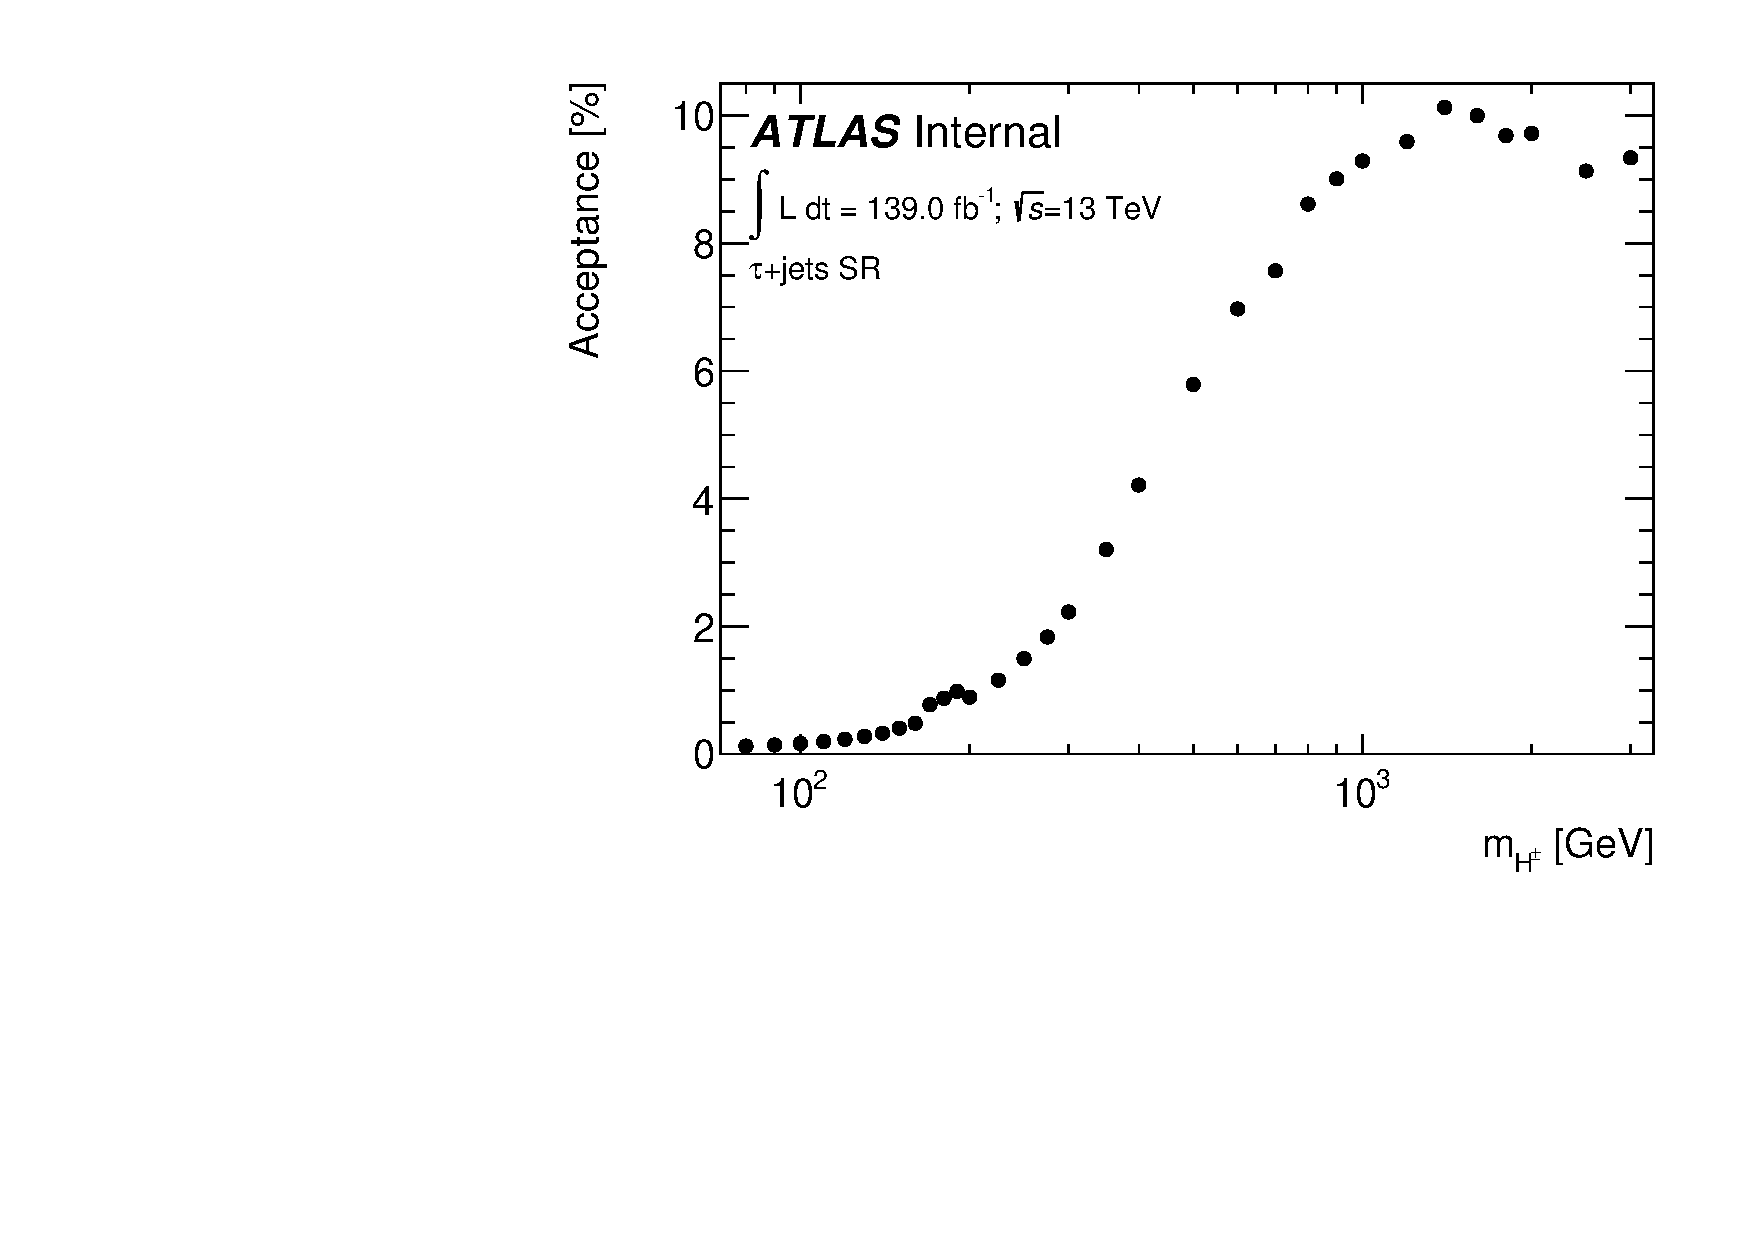
\includegraphics[width=0.5\textwidth]{chapters/chapter6_HPlus/images/Signal_Acceptance_Efficiency_SR_TAUJET.pdf}}
				\subfloat[\label{fig:signal-acceptance_b}]{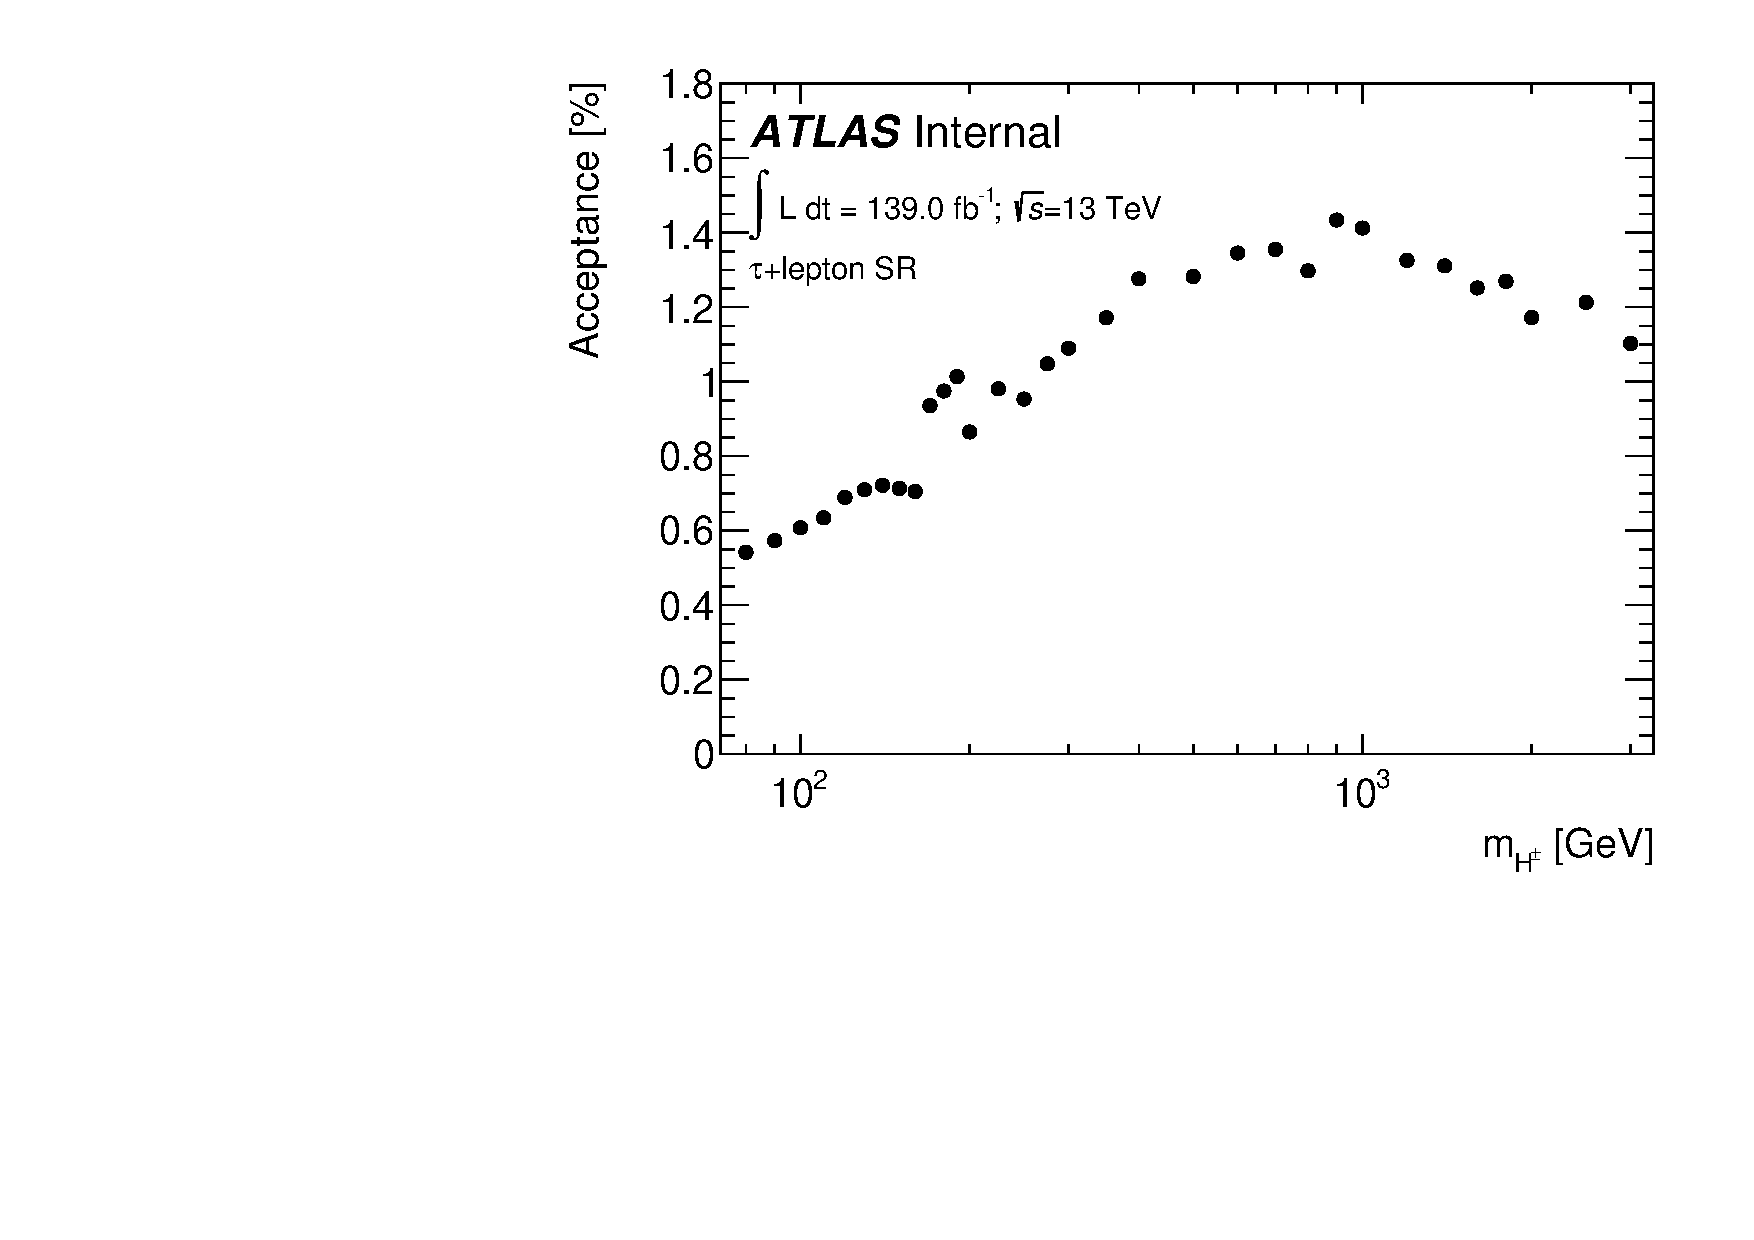
\includegraphics[width=0.5\textwidth]{chapters/chapter6_HPlus/images/Signal_Acceptance_Efficiency_SR_TAULEP.pdf}}
				\caption{\label{fig:signal-acceptance} Signal acceptance as a function of the charged Higgs boson mass for both the \taujets (a) and \taulep subchannels (b).}
			\end{figure}

	\section{Datasets}\label{sec:datasets}
		This analysis uses the full Run-2 ATLAS dataset collected between 2015 and 2018 corresponding to $139.0 \pm 2.4$ \ifb \cite{lumi-run2}. The datasets used are required to be included in the ATLAS ``Good Run Lists'' (GRLs), meaning they have passed nominal data quality checks with all detector subsystems operating within normal conditions. Further event cleaning is applied that removes events in which a reconstructed jet originated from detector noise or non-collision backgrounds. The collection of data throughout Run-2 can be seen in Figure \ref{fig:lhc-lumi}.

		\subsection{Signal Modeling}\label{ssec:sig-modeling}
		Monte Carlo (MC) simulations of \Hpm signal events are generated at varying orders dependent on \mHpm. In all cases, the 2HDM Type II model described in Section \ref{ssec:2HDM} is assumed and the generator MadGraph is used. The lower mass range corresponding to $\mHpm < 140$ GeV where a \Hpm takes the place of a $W^{\pm}$ in a top decay is generated at LO. The intermediate mass range of $140 \leq \mHpm < 200 $ GeV is generated at LO, taking into account the non-resonant, single-top resonant and double-resonant diagrams and their interferences. In this mass range, the final state contains one \Hpm, one $W^{\pm}$, and two b quark. For charged Higgs masses of 200 GeV and above, the \Hpm is produced in association with a top quark and is generated at NLO. In all cases, the parton generator is interfaced with Pythia 8 using the A14 underlying event tuning parameters \cite{Pythia8-tunes}. Table \ref{tab:signal-generated} shows the cross section and raw number of events generated for each \mHpm point for both subchannels.

		\begin{table}[!thp]
			\centering
			\resizebox{.65\textwidth}{!}{
			\begin{tabular}{| l | l | l | l |}
			\hline
			\mHpm [GeV] 	& $\sigma$ [pb] 	& \taulep Generated Events 	& \taujets Generated Events 	\\ \hline
			80 				& 61.639 			& 220k 						& 110k							\\
			90 				& 52.823 			& 220k 						& 110k							\\
			100 			& 43.777 			& 220k 						& 110k							\\
			110				& 34.770 			& 220k 						& 110k							\\
			120 			& 26.092 			& 220k 						& 110k							\\
			130 			& 18.069 			& 220k 						& 110k							\\ \hline
			140 			& 15.023 			& 220k 						& 220k							\\
			150 			& 7.681 			& 220k 						& 220k							\\
			160 			& 2.665 			& 220k 						& 220k							\\
			170 			& 0.63748 			& 220k 						& 220k							\\
			180 			& 0.52979 			& 220k 						& 220k							\\
			190 			& 0.47201 			& 220k 						& 220k							\\ \hline
			200 			& 0.55632 			& 110k 						& 220k							\\
			225 			& 0.44081 			& 110k 						& 220k							\\
			250 			& 0.3573 				& 110k 						& 220k							\\
			275 			& 0.28592 			& 110k 						& 220k							\\
			300 			& 0.23373 			& 110k 						& 220k							\\
			350 			& 0.15774 			& 110k 						& 220k							\\
			400 			& 0.10818 			& 110k 						& 220k							\\
			500 			& 0.054139 			& 110k 						& 220k							\\
			600 			& 0.02847 			& 110k 						& 220k							\\
			700 			& 0.015764 			& 110k 						& 220k							\\
			800 			& 0.009067 			& 110k 						& 220k							\\
			900 			& 0.005324 			& 110k 						& 220k							\\
			1000 			& 0.003271 			& 110k 						& 220k							\\
			1200 			& 0.001311 			& 110k 						& 220k							\\
			1400 			& 0.000558 			& 110k 						& 220k							\\
			1600 			& 0.000252 			& 110k 						& 220k							\\
			1800 			& 0.000120 			& 110k 						& 220k							\\
			2000 			& 0.0000587 		& 110k 						& 220k							\\
			2500 			& 0.0000111			& 110k 						& 220k							\\
			3000 			& 0.00000234		& 110k 						& 220k							\\ \hline
			\end{tabular}}
			\caption{For each \Hpm mass the generator xcross-section $(\sigma \times BR(\HpmLong))$ is given, as well as the number of generated events for both \taulep and \taujets subchannels.}
			\label{tab:signal-generated}
		\end{table}
		% \pagebreak

	\section{Background Modeling}\label{sec:bkg-modeling}
		The main sources of backgrounds are shown in Table \ref{tab:backgrounds}, separated between backgrounds with a prompt \tauhad in the hard scatter process and those that arise from the misidentification of other physics objects as a \tauhad. The cross section of all simulated background samples and the relevant generators can be seen in Table \ref{tab:bkg-xs}. Control regions that are designed to be orthogonal to the signal region are created for both subchannels in order to study the modeling of the backgrounds. These control regions are defined by the cuts in Table \ref{tab:taujet-control-regions} (\taujets) and Table \ref{tab:taulep-control-regions} (\taulep). For the \taulep subchannel the Same Sign and b-veto control regions are further split into two control regions, one that requires a $\mu$ in the event and another that requires an electron. The \Etm distributions in each of the control regions are plotted in Figure \ref{fig:bkg-met-taujets} (\taujets) and Figure \ref{fig:bkg-met-taulep} (\taulep). These plots include a ratio of reconstructed data events and simulated MC events bin by bin to ensure proper modeling. More background modeling plots can be seen in Appendix \ref{app:valid-plots}.

		As seen in Table \ref{tab:backgrounds} misidentified objects appearing as \tauhad candidates comprise a significant portion of the total background. Fakes arising from $\ell \rightarrow \tau$ misidentification are well modeled in MC simulations and are reweighted with scale factors provided by the ATLAS $\tau$ combined performance group. The mass of the \tauhad electron system can be seen in Figure \ref{fig:zee-mass} as verification of fake $\ell \rightarrow \tau$ modeling.

    \begin{table}[!thp]
      \centering
      \resizebox{\textwidth}{!}{
      \begin{tabular}{| l | l |}
      \hline
      Backgrounds w/ prompt \tauhad & Backgrounds w/ fake $\tau$ \\
      \hline \hline
      $t\bar{t}$ estimated with MC       & Fake $j \rightarrow \tau$ estimated with data driven fake factor method \\ \hline
      $W(Z)+jets$ estimated with MC         & Fake $\ell \rightarrow \tau$ estimated with MC, validated on $Z \rightarrow ee$\\ \hline
      Diboson estimated with MC & \\
      \hline
      \end{tabular}}
      \caption{Dominant backgrounds from prompt \tauhad and fake \tauhad candidates.}
      \label{tab:backgrounds}
    \end{table}

		\begin{table}[!thp]
			\begin{center}
			\small
			\resizebox{0.5\textwidth}{!}{
			\begin{tabular}{|c||c|c|}
			\hline
			Background process & Generator \& & Cross section \\
			  & parton shower & number(s) [pb] \\
			\hline \hline
			$\begin{array}{c}
			$\ttbar$~\mbox{with at least one lepton $\ell$} \\ 
			\end{array}$ &
			$\begin{array}{c}
			\mbox{{\textsc Powheg}}~\& \\
			\mbox{{\textsc Pythia8}}
			\end{array}$
			& 729.77* \\
			\hline
			$\begin{array}{c}
			\mbox{Single top-quark}\\ 
			\mbox{$t$-channel}
			\end{array}$ & & 59.17* \\
			$\begin{array}{c}
			\mbox{Single top-quark}\\ 
			\mbox{$s$-channel}
			\end{array}$ &
			$\begin{array}{c}
			\mbox{{\textsc Powheg}}~\& \\
			\mbox{{\textsc Pythia8}}
			\end{array}$ & 3.29* \\
			$\begin{array}{c}
			\mbox{Single top-quark}\\ 
			\mbox{$Wt$-channel}
			\end{array}$  & & 83.83  \\
			\hline
			$\begin{array}{c}
			~ \\
			W(\ell\nu) + \mbox{jets} \\ 
			~ \\
			\end{array}$ &
			$\begin{array}{c}
			~ \\
			\mbox{Sherpa 2.2.1} \\ 
			~ \\
			\end{array}$ &
			$\begin{array}{c}
			2.0\times 10^4 \\
			2.0\times 10^4 \\ 
			2.0\times 10^4 \\
			\end{array}$ \\
			\hline
			$\begin{array}{c}
			Z/\gamma^{\ast}(\ell\ell,\nu\nu) + \mbox{jets} \\
			\end{array}$ & 
			$\begin{array}{c}
			~ \\
			\mbox{Sherpa 2.2.1} \\ 
			~ \\
			\end{array}$  &
			$\begin{array}{c}
			2.1 \times 10^3  \\
			2.1 \times 10^3  \\ 
			2.1 \times 10^3  \\
			\end{array}$ \\

			\hline
			$WW$  &  & 54.81 \\
			$WZ$  &  $\begin{array}{c}
			\mbox{{\textsc Powheg}}~\& \\
			\mbox{{\textsc Pythia8}}
			\end{array}$ & 16.34 \\
			$ZZ$  &  & 8.94 \\
			\hline
			\end{tabular}}
			\normalsize
			\caption{\label{tab:bkg-xs}
			Cross sections for the main SM 
			background samples at \sqs. 
			Here, $\ell$ refers to the three lepton families $e$, $\mu$ and 
			$\tau$. All background cross sections are normalised to NNLO predictions, 
			except for diboson events, where the NLO prediction is used. A '*' indicates
			that the quoted cross section for the sample is neglecting leptonic/hadronic
			branching ratios.
			}
			\end{center}
		\end{table}

		\begin{table}[!thp]
			\begin{subtable}[c]{0.45\textwidth}
				\centering
				\begin{tabular}{| c |}
					\hline
        	\textbf{\ttbar Control Region} \\ \hline \hline
          1 \tauhad \\
          $\pt^{\tau} > 40 $ GeV \\
          $\geq 3 $ jets\\
          $\geq 2 $ \bjets\\
          $\Etm > 150 GeV$ \\
          $m_{T}(\tau, \Etm) < 100 \: GeV$ \\
          \hline
				\end{tabular}
				\subcaption{\ttbar modeling}
			\end{subtable}
			\begin{subtable}[c]{.45\textwidth}
				\centering
				\begin{tabular}{| c |}
					\hline
					\textbf{b-veto Control Region} \\ \hline \hline
					1 \tauhad \\
					$\pt^{\tau} > 40 \: GeV $  \\
					$\geq 3$ jets\\
					% $n\_bjets > 2$ \\
					$\pt^{jet} > 25 \: GeV$ \\
					$\Etm > 150 GeV$ \\
					$m_{T}(\tau, \Etm) > 50 \: GeV$ \\
					b veto \\
					$\ell$ veto \\
					\hline
				\end{tabular}
				\subcaption{Close to signal region}
			\end{subtable}
			\begin{subtable}[c]{.45\textwidth}
				\centering
				\begin{tabular}{| c |}
					\hline
					\textbf{W+Jets Control Region} \\ \hline \hline
					1 \tauhad \\
					$\pt^{\tau} > 40 \: GeV $  \\
					$\geq 3$ jets \\
					$\pt^{jet} > 25 \: GeV$ \\
					$\Etm > 150 GeV$ \\
					$m_{T}(\tau, \Etm) > 100 \: GeV$ \\ 
					b veto \\
					$\ell$ veto \\
					\hline
				\end{tabular}
				\subcaption{W+Jets modeling}
			\end{subtable}
			\begin{subtable}[c]{.45\textwidth}
				\centering
				\begin{tabular}{| c |}
					\hline
					\textbf{b-veto $m_{T}\geq100$ Control Region} \\ \hline \hline
					1 \tauhad \\
					$\pt^{\tau} > 40 \: GeV $  \\
					$\geq 3$ jets \\
					$\pt^{jet} > 25 \: GeV$ \\
					$\Etm > 150 GeV$ \\
					$m_{T}(\tau, \Etm) > 100 \: GeV$ \\
					b veto \\
					$\ell$ veto \\
					\hline
				\end{tabular}
				\subcaption{Fake $j \rightarrow \tau$ enriched region}
			\end{subtable}

			\caption{Control region definitions for the \taujets subchannel.}
			\label{tab:taujet-control-regions}
		\end{table}

		\begin{table}[!thp]
			\begin{subtable}[c]{0.45\textwidth}
				\centering
				\begin{tabular}{| c |}
					\hline
        	\textbf{Dilepton-btag CR} \\ \hline \hline
          $\tau$ veto \\
          $n\geq 1$ jets \\
          $\pt^{jet} > 25 GeV$ \\
          $\geq 1$ \bjets \\
          $\Etm > 50 GeV$ \\
          1 $e$ \\
          1 $\mu$ \\
          \hline
				\end{tabular}
				\subcaption{\ttbar and single top modeling}
			\end{subtable}
			\begin{subtable}[c]{.45\textwidth}
				\centering
				\begin{tabular}{| c |}
					\hline
	        \textbf{b-veto CR} \\ \hline \hline
          1 \tauhad \\
          $\pt^{\tau} > 30 \: GeV $  \\
          1 $e (\mu) $ \\
          Veto $\mu \:(e)$ \\
          Opposite sign $\tau$ $e \: (\mu)$ \\
          $\geq 1$ jets  \\
          $\pt^{jet} > 25 GeV$ \\
          $\Etm > 50 GeV$ \\
          1 tight $e \: (\mu)$ \\
          \hline					
				\end{tabular}
				\subcaption{Close to signal region}
			\end{subtable}
			\begin{subtable}[c]{.45\textwidth}
				\centering
				\begin{tabular}{| c |}
					\hline
        	\textbf{Zee CR} \\ \hline \hline
          1 \tauhad \\
          $\pt^{\tau} > 30 \: GeV $  \\
          veto $\mu$ \\
          Opposite sign $\tau$ $e$ \\
          $\geq 1$ jets \\
          $\pt^{jet} > 25 GeV$ \\
          \bjet veto \\
          $\Etm > 50 GeV$ \\
          1 $e$\\
          $40 < mass(\tau,e) < 140 GeV$ \\
          \hline
				\end{tabular}
				\subcaption{Fake $\ell \rightarrow \tau$ enriched region}
			\end{subtable}
			\begin{subtable}[c]{.45\textwidth}
				\centering
				\begin{tabular}{| c |}
					\hline
	        \textbf{Same Sign CR} \\ \hline \hline
          1 \tauhad \\
          $\pt^{\tau} > 30 \: GeV $  \\
          Same sign $\tau \: e(\mu)$ \\
          Veto $\mu\:(e)$ \\
          $\geq 1 jets$ \\
          $\pt^{jet} > 25 GeV$ \\
          $\Etm > 50 GeV$  \\
          1 tight $e \: (\mu)$ \\
          \hline
				\end{tabular}
				\subcaption{Fake $j \rightarrow \tau$ enriched region}
			\end{subtable}

			\caption{Control region definitions for the \taulep subchannel.}
			\label{tab:taulep-control-regions}
		\end{table}

		\pagebreak
		\begin{figure}[!thp]
			\begin{center}    
			% 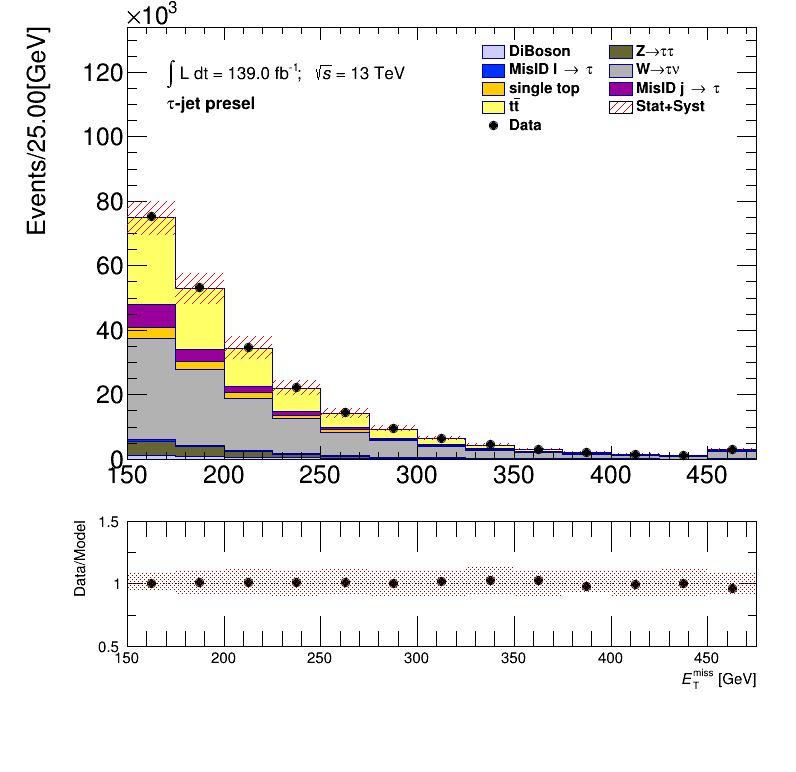
\includegraphics[width=0.45\textwidth]{chapters/chapter6_HPlus/images/taujets/met_et_TAUJET_PRESEL.png} \\
			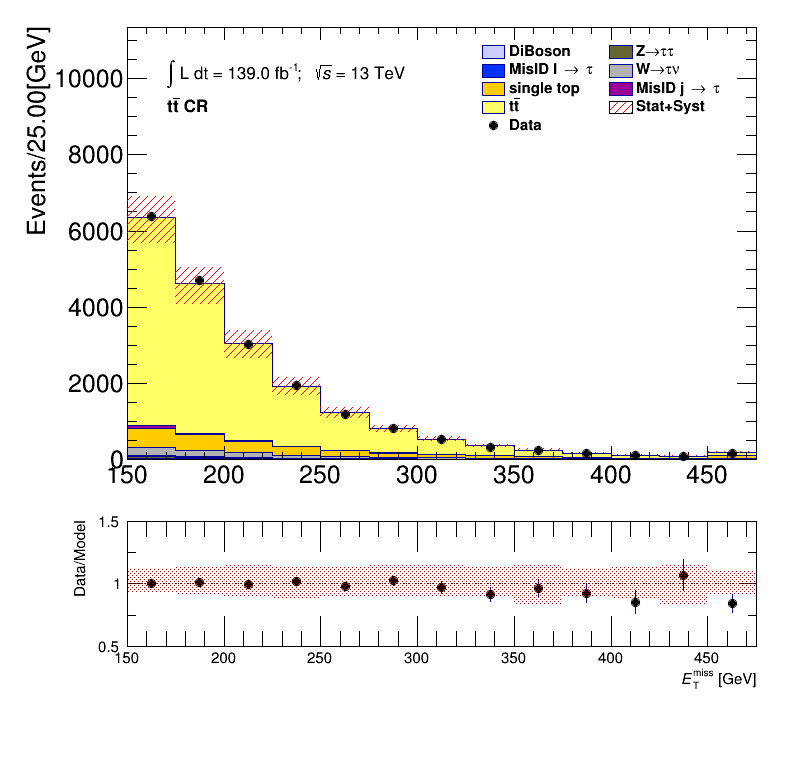
\includegraphics[width=0.45\textwidth]{chapters/chapter6_HPlus/images/taujets/met_et_TTBAR.png}
			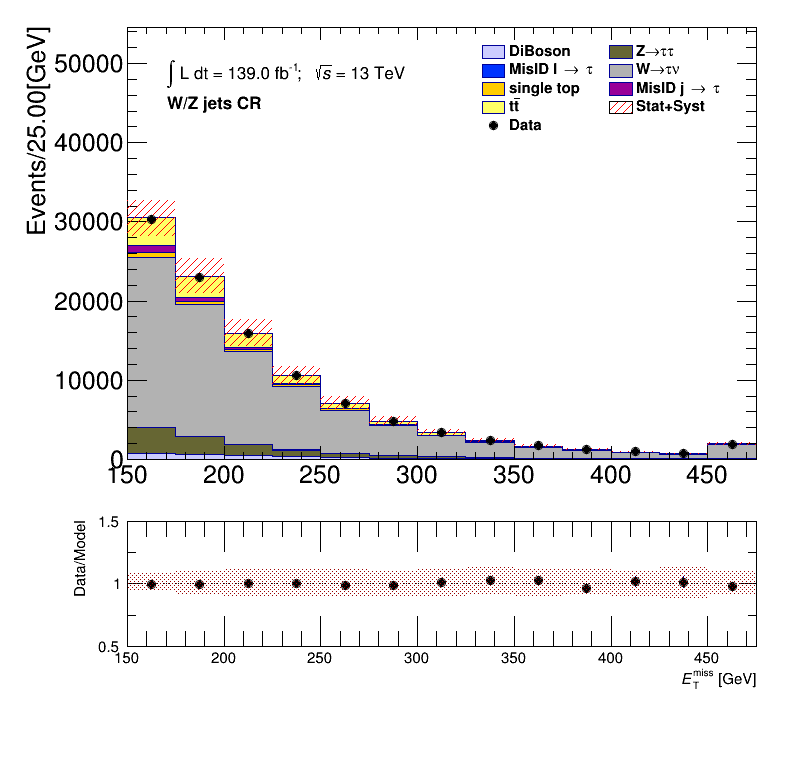
\includegraphics[width=0.45\textwidth]{chapters/chapter6_HPlus/images/taujets/met_et_WJETS.png} \\
			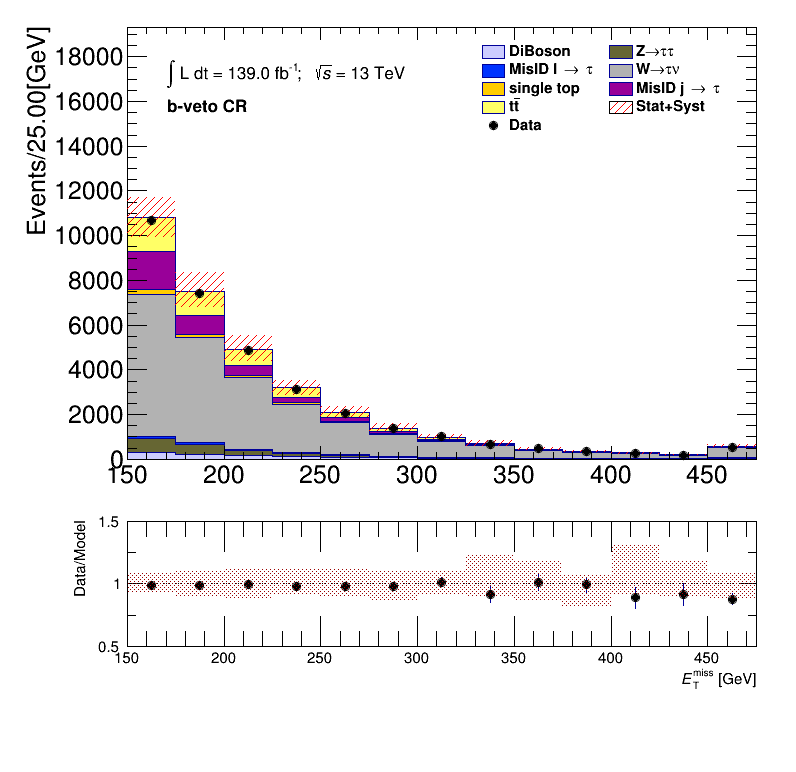
\includegraphics[width=0.45\textwidth]{chapters/chapter6_HPlus/images/taujets/met_et_BVETO.png}
			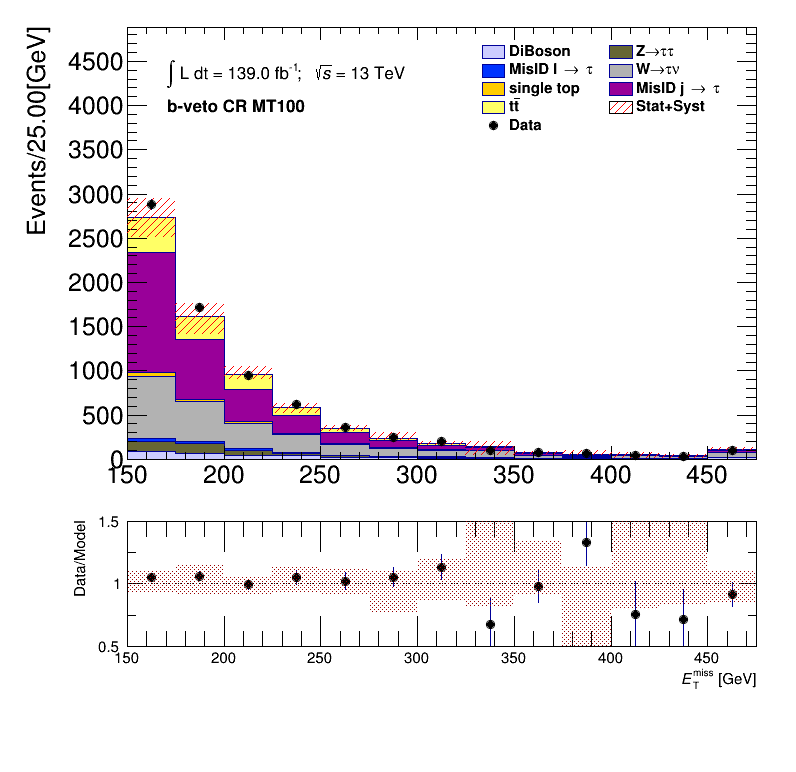
\includegraphics[width=0.45\textwidth]{chapters/chapter6_HPlus/images/taujets/met_et_BVETO_MT100.png} \\
			\end{center}
			\caption{
			Comparison between the predicted and the measured \Etm distributions in various control regions defined for the \taujets channel. The uncertainty band includes both statistical and systematic uncertainties on the background prediction. 
			}
			\label{fig:bkg-met-taujets}
		\end{figure}

		\pagebreak
		\begin{figure}[!thp]
			\begin{center}    
			% 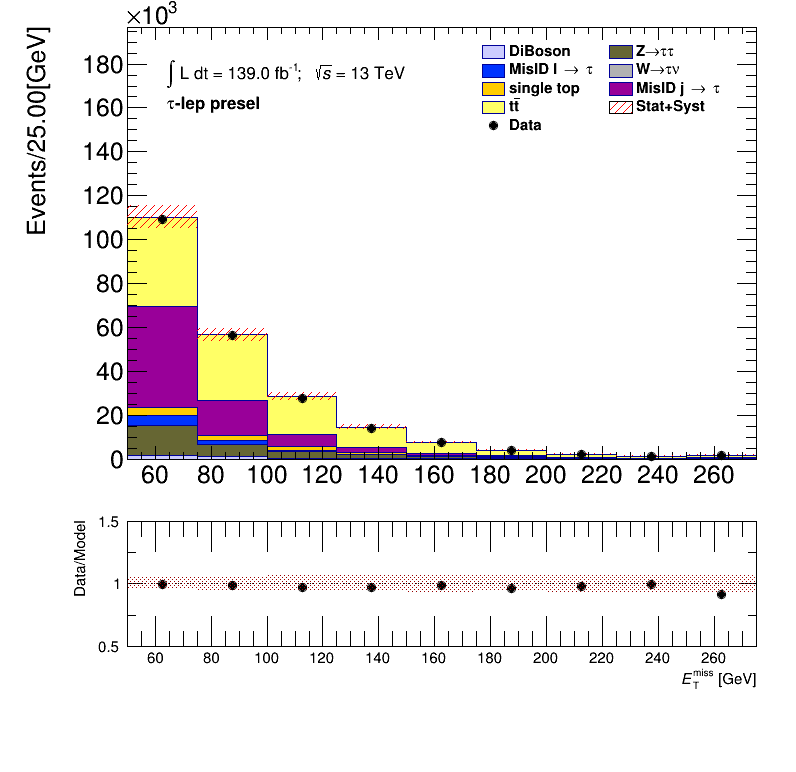
\includegraphics[width=0.45\textwidth]{chapters/chapter6_HPlus/images/taulep/met_et_TAULEP_PRESEL.png} \\
			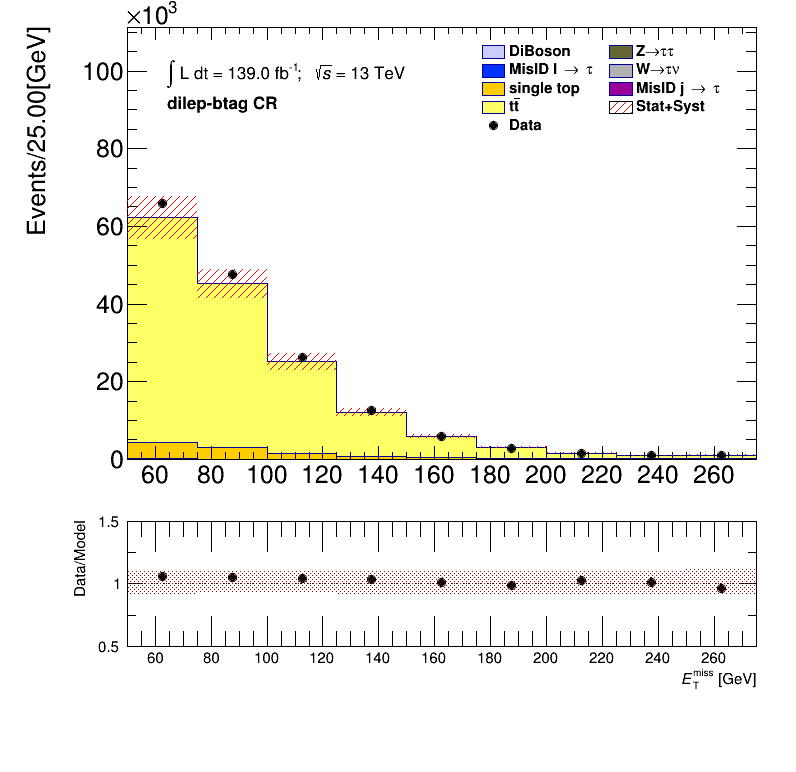
\includegraphics[width=0.45\textwidth]{chapters/chapter6_HPlus/images/taulep/met_et_DILEP_BTAG.png}
			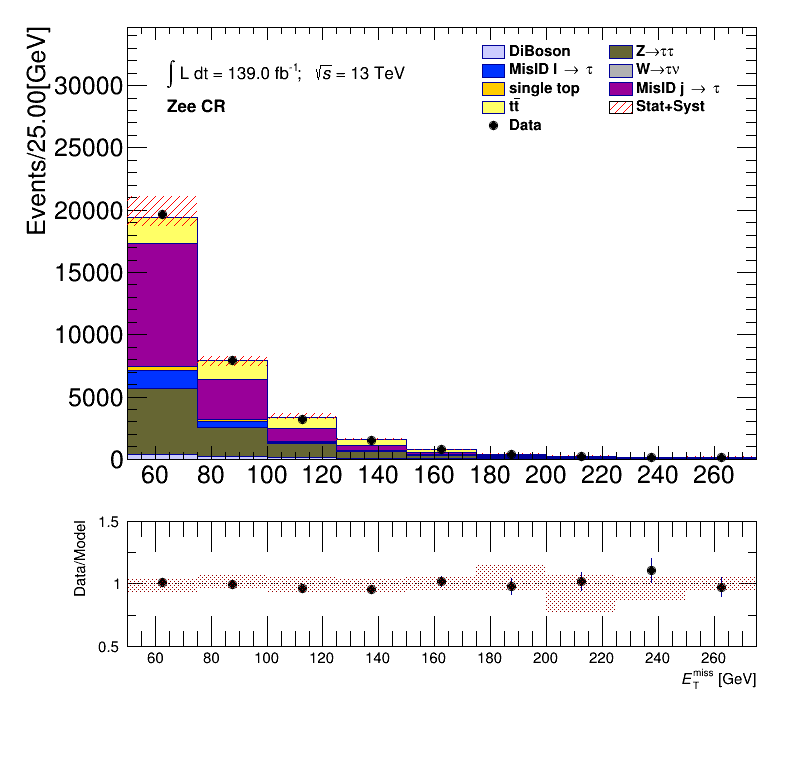
\includegraphics[width=0.45\textwidth]{chapters/chapter6_HPlus/images/taulep/met_et_ZEE.png} \\
			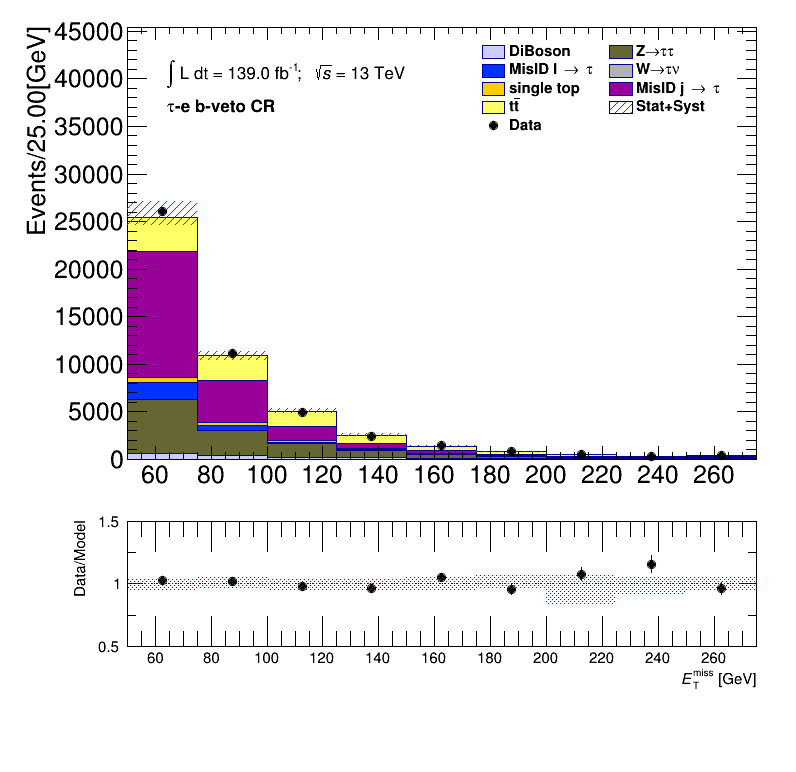
\includegraphics[width=0.45\textwidth]{chapters/chapter6_HPlus/images/taulep/met_et_TAUEL_BVETO.png} 
			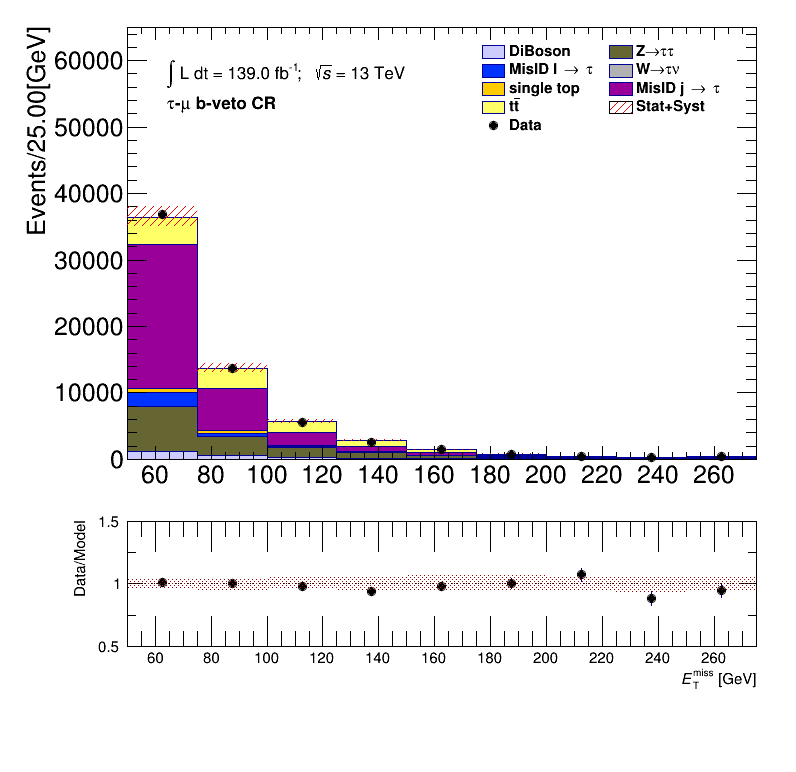
\includegraphics[width=0.45\textwidth]{chapters/chapter6_HPlus/images/taulep/met_et_TAUMU_BVETO.png} \\
			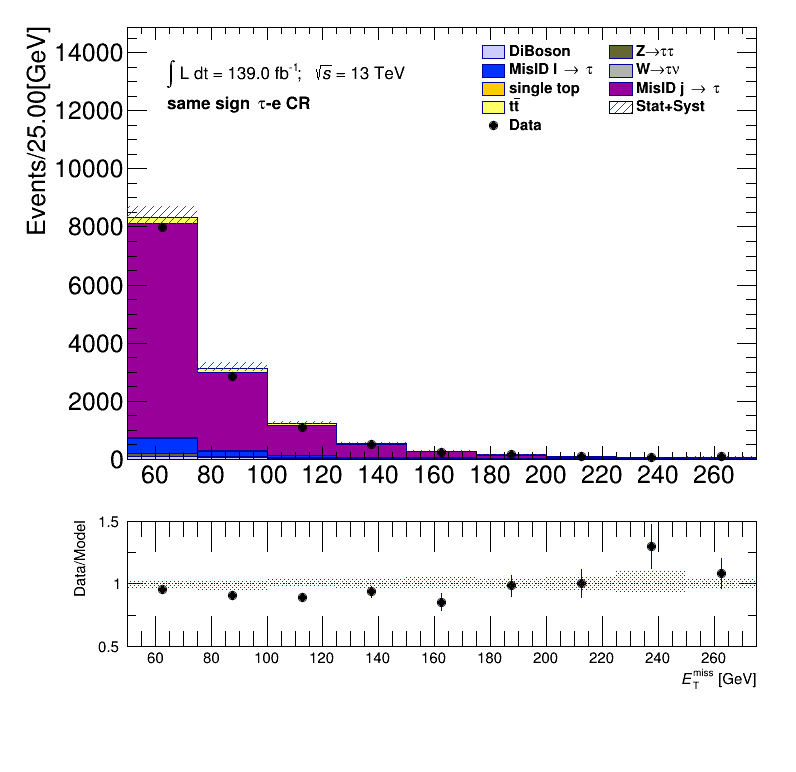
\includegraphics[width=0.45\textwidth]{chapters/chapter6_HPlus/images/taulep/met_et_SS_TAUEL.png} 
			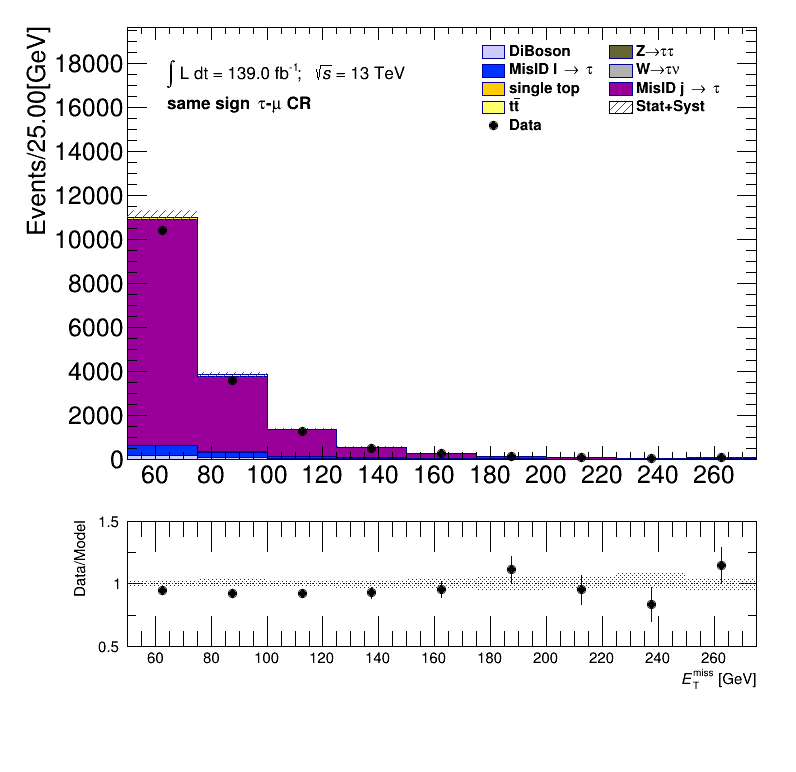
\includegraphics[width=0.45\textwidth]{chapters/chapter6_HPlus/images/taulep/met_et_SS_TAUMU.png} \\
			\end{center}
			\caption{
			Comparison between the predicted and the measured \Etm distributions in various control regions defined for the \taulep channel. The uncertainty band includes both statistical and systematic uncertainties on the background prediction. 
			}
			\label{fig:bkg-met-taulep}
		\end{figure}

		\begin{figure}[!thp]
			\centering
			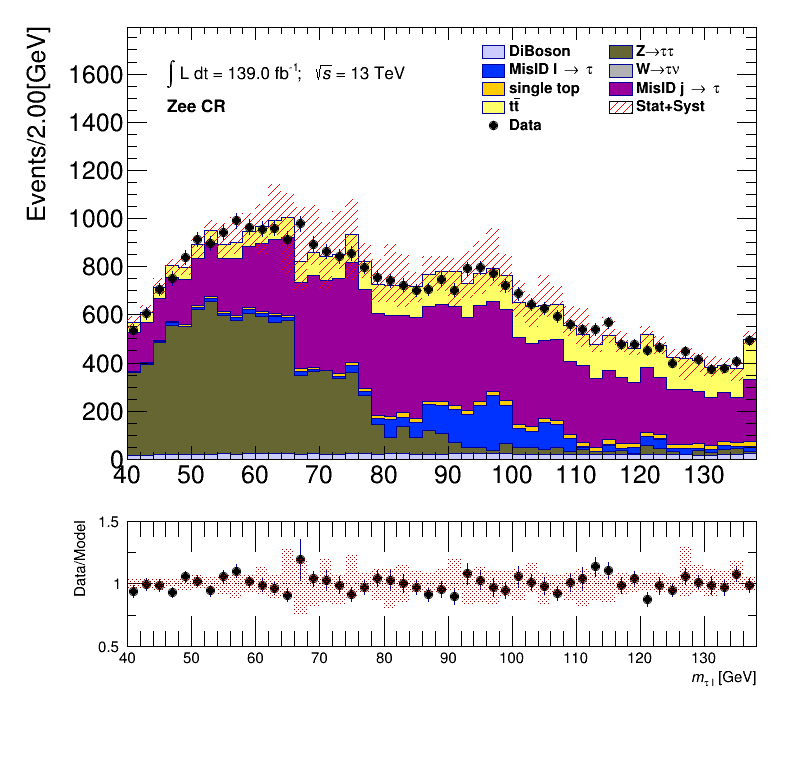
\includegraphics[width=.5\textwidth,keepaspectratio=true]{chapters/chapter6_HPlus/images/taulep/tau_0_lep_0_mass_ZEE.png}
			\caption{Mass of $\tau$ - e system in the Zee control region.}
			\label{fig:zee-mass}
		\end{figure}

	\section{Analysis Strategy}\label{sec:ana-strat}

		\subsection{Multivariate Analysis Techniques}\label{ssec:mva}

		\subsection{Training}\label{ssec:training}

		\subsection{Feature Selection}\label{ssec:features}

		\subsection{Hyperparameter Optimization}\label{ssec:hpo}

	\section{Systematic Uncertainties}\label{sec:systs}

	\section{Results}\label{sec:results}

